\documentclass{article}

\usepackage{graphicx}

\begin{document}
\title{Homework 16}
\date{}
\maketitle

% 1. Fall 2011, #11
% 2. Spring 2012, #11
% 3. Fall 2012, #6

\paragraph{\Large 1. Fall 2011 Final Question 11}\mbox{}\\
Consider the following \textit{st}-flow network and feasible flow \textit{f}.\\
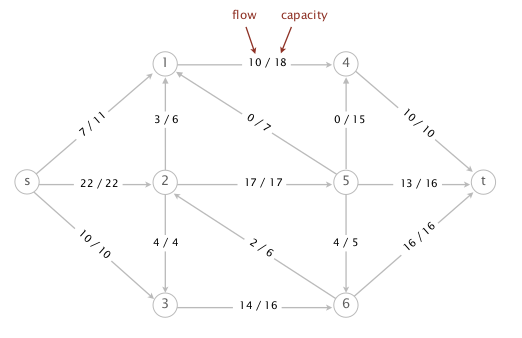
\includegraphics[]{fin-f11-11.png}\\
\begin{enumerate}
\renewcommand{\theenumi}{\Alph{enumi}}
	\item What is the value of the flow \textit{f}?.\\
	
	39

	\item Perform one iteration of the Ford-Fulkerson algorithm, starting from the flow \textit{f}. Give the sequence of vertices on the augmenting path.\\

	$s$, 1, 2, 6, 5, $t$  

	\item What is the value of the maximum flow \textit{f}?.\\
	
	$16 + 10 + 15 = 41$

	\item List the vertices on the \textit{s} side of the minimum cut.\\

	1, 2, 4

	\item What is the capacity of the minimum cut?

	41

\end{enumerate}


\paragraph{\Large 2. Spring 2012 Final Question 1}1\mbox{}\\
Run the eager version of Dijkstra’s algorithm on the following edge-weighted digraph, starting from vertex 0.\\
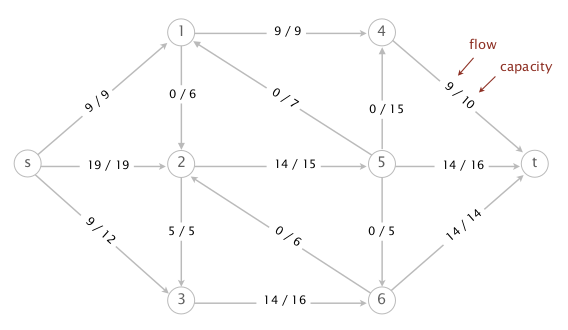
\includegraphics[]{fin-s12-11.png}
\begin{enumerate}
\renewcommand{\theenumi}{\Alph{enumi}}
	\item What is the value of the flow \textit{f}?.\\
	
	37

	\item Perform one iteration of the Ford-Fulkerson algorithm, starting from the flow \textit{f}. Give the sequence of vertices on the augmenting path.\\

	$s$, 3, 6, 2, 5, $t$  

	\item What is the value of the maximum flow \textit{f}?.\\
	
	$37+1=38$

	\item List the vertices on the \textit{s} side of the minimum cut.\\

	2, 3, 6

	\item What is the capacity of the minimum cut?

	38

\end{enumerate}


\paragraph{\Large 3. Fall 2012 Final Question 6}1\mbox{}\\
Consider the following flow network and feasible flow $f$ from from the source vertex $A$ to the sink vertex $J$.\\
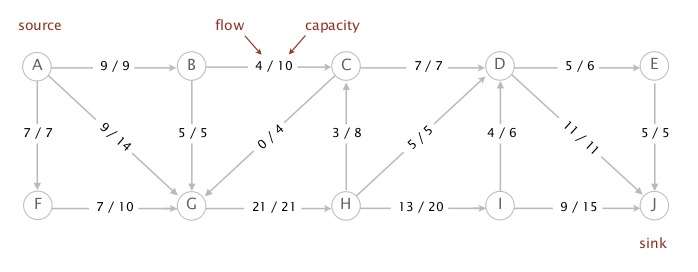
\includegraphics[width=\linewidth]{fin-f12-6.png}
\begin{enumerate}
\renewcommand{\theenumi}{\Alph{enumi}}
	\item What is the value of the flow \textit{f}?.\\
	
	25

	\item Starting from the flow $f$ given above, perform one iteration of the Ford-Fulkerson algorithm. List the sequence of vertices on the augmenting path.\\

	$A, G, B, C, H, I, J$

	\item What is the value of the maximum flow \textit{f}?.\\
	
	$25+3=28$

	\item List the vertices on the source side of the minimum cut in alphabetical order.\\

	$A, B, C, F, G$

	\item What is the capacity of the minimum cut?

	28

\end{enumerate}

\end{document}